\section{Methodology}

The overall workflow of the system is shown in Figure~\ref{fig:system-architecture}.

\begin{figure}[htbp]
    \centering
    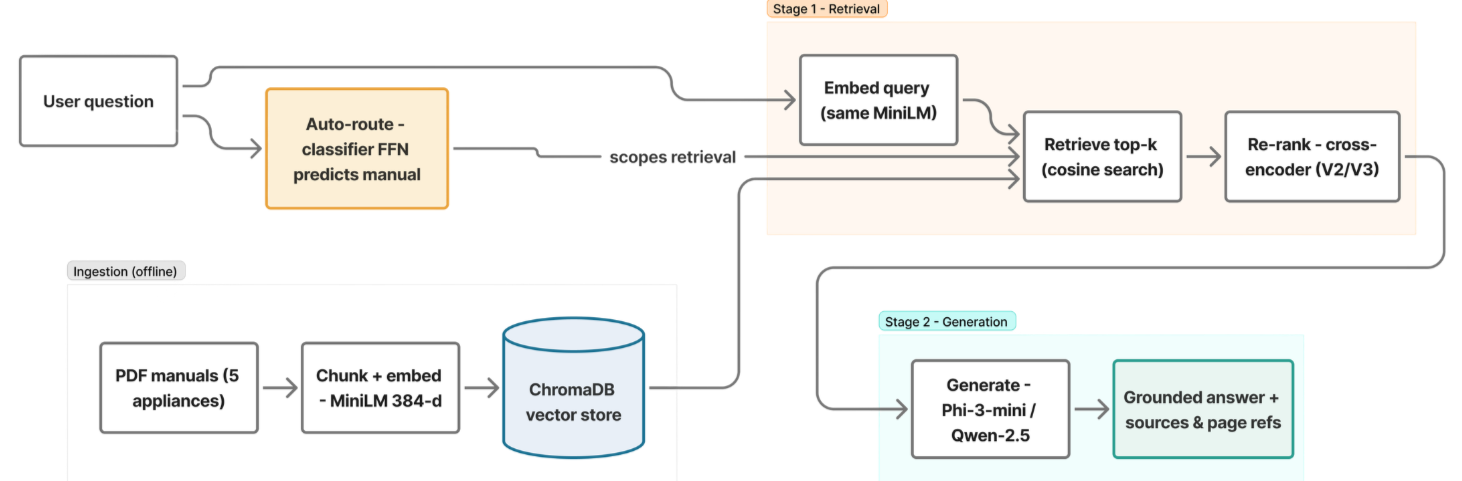
\includegraphics[width=\textwidth]{figures/system_archi.png}
    \caption{System architecture of the retrieval-augmented chatbot for product manuals.}
    \label{fig:system-architecture}
\end{figure}

\subsection{Manual Ingestion and Text Processing}

The product manuals were stored as PDF files inside the \texttt{backend/manuals/} directory. The system used the \texttt{pypdf} library to extract text from each PDF page. During extraction, whitespace and repeated line breaks were normalized to reduce formatting noise from the original manuals.

After text extraction, each page was divided into overlapping text chunks. In the final retrieval setup, the chunk size was set to 500 characters with an overlap of 80 characters. This overlap was used so that important information near chunk boundaries would not be completely separated. Each chunk was stored together with its source filename and page number as metadata.

\subsection{Manual Corpus}

The system used five product manuals as its document corpus as shown in Table~\ref{tab:manual-corpus}. These manuals were placed in the \texttt{backend/manuals/} directory and were indexed for retrieval. 

\begin{table}[htbp]
\centering
\caption{Product manuals included in the RAG corpus}
\label{tab:manual-corpus}
\small
\setlength{\tabcolsep}{4pt}
\renewcommand{\arraystretch}{1.15}

\begin{tabularx}{\textwidth}{@{}p{2.4cm}Y p{4.1cm}@{}}
\toprule
\textbf{Category} & \textbf{Manual} & \textbf{Filename} \\
\midrule

Air conditioner &
Panasonic Air Conditioner Service Manual for CS-NZ25YKE, CS-NZ35YKE, CS-NZ50YKE, CU-NZ25YKE, CU-NZ35YKE, and CU-NZ50YKE &
\texttt{Service-Manual-18.pdf} \\

Printer &
HP LaserJet Pro MFP M329, M428--M429 User Guide &
\texttt{c06184015.pdf} \\

Printer &
Epson ET-4850 User's Guide &
\texttt{cpd60205.pdf} \\

Refrigerator &
Samsung Refrigerator User Manual for RF32CG, RF27CG, and RF70F27 series &
\begin{minipage}[t]{4.1cm}
\ttfamily\footnotesize
DA68-04752Q\_FDR\_RF6500C\_\\3Door\_EN\_MES\_CFR\_260209.pdf
\end{minipage} \\

Washing machine &
LG Washing Machine Owner's Manual for WM4200H*A and WM4000H*A &
\texttt{db05a9.pdf} \\

\bottomrule
\end{tabularx}
\end{table}

\subsection{Embedding and Vector Storage}

Each text chunk was converted into a dense vector representation using the \texttt{sentence-transformers} library. The final embedding model used for retrieval was \texttt{BAAI/bge-small-en-v1.5}, which produces 384-dimensional embeddings. The embeddings were normalized so that cosine similarity could be used during vector search.

The vector embeddings, chunk text, source filename, and page metadata were stored in a persistent \texttt{ChromaDB} collection. The ChromaDB collection was configured to use cosine similarity for comparing query and document embeddings.

\subsection{Retrieval and Re-ranking}

In the final setup, the retriever first obtains up to 20 candidate chunks from ChromaDB.

To improve the quality of the retrieved context, the system applies a second-stage re-ranking process using the \texttt{cross-encoder/ms-marco-MiniLM-L-6-v2} model. Unlike the embedding model, which compares query and document vectors separately, the cross-encoder evaluates each query-chunk pair together and assigns a relevance score. The system then sorts the retrieved candidates by this score and returns the top \texttt{k} chunks, with \texttt{top\_k = 4} used as the default setting.

The retrieval process also supports source filtering. If a specific manual filename is provided, ChromaDB only retrieves chunks from that manual. This prevents the chatbot from mixing information from different appliance manuals.

\subsection{Answer Generation}

The retrieved chunks are passed to a generator model, which produces the final natural-language answer. The generator was implemented in \texttt{generator.py} with two interchangeable backends.

The first backend uses Hugging Face Transformers with PyTorch to run \texttt{microsoft/Phi-3-mini-4k-instruct}. This served as the main generator for the baseline and improved retrieval variants. The second backend uses a local Ollama server through the endpoint \texttt{http://localhost:11434/api/generate}, with \texttt{qwen2.5:3b} as the generator model.

Both generator backends use the same system prompt. The prompt instructs the model to answer only from the retrieved manual context, avoid unsupported claims, avoid telling the user to consult the manual, and avoid adding filenames or page numbers inside the generated answer. The system uses greedy decoding by setting the temperature to 0.0 to make responses more consistent for factual manual-based question answering.

After generation, the response is passed through a post-processing step in \texttt{rag\_pipeline.py}. This step removes any model-generated inline citations such as fabricated filename-page references. Instead of relying on the model to cite sources, the system returns structured source records based on retriever metadata.

\subsection{API and Frontend Implementation}

The backend was implemented using \texttt{FastAPI}. The API was run locally using \texttt{Uvicorn}. The main API endpoints were:

\begin{enumerate}
    \item \texttt{GET /health} -- checks whether the backend is running.
    \item \texttt{GET /sources} -- returns the list of indexed manual filenames.
    \item \texttt{POST /ingest} -- rebuilds the ChromaDB index from the PDF manuals.
    \item \texttt{POST /ask} -- performs retrieval and answer generation.
    \item \texttt{POST /classify} -- predicts which manual a query belongs to.
    \item \texttt{POST /ask\_auto} -- automatically classifies the query, routes it to the predicted manual, and generates an answer.
\end{enumerate}

The frontend was developed using Vite and React. It provides a chat interface where users can type questions, select the generator backend, and view the generated answer with its retrieved sources. The frontend first calls the classifier endpoint to route the query, then sends the question to the \texttt{/ask} endpoint using the predicted manual as the source filter.

\subsection{Manual Classification}

To reduce the need for users to manually select a product manual, the system includes a manual classifier implemented in \texttt{manual\_classifier.py}. The classifier uses frozen \texttt{sentence-transformers/all-MiniLM-L6-v2} embeddings as input. The embedding output is a 384-dimensional vector.

A small feed-forward neural network was trained on top of these frozen embeddings. The classifier architecture was:

\[
\text{Linear}(384 \rightarrow 128) \rightarrow \text{ReLU} \rightarrow \text{Dropout}(0.2) \rightarrow \text{Linear}(128 \rightarrow 5)
\]

The five output classes correspond to the five appliance manuals. The output logits are passed through a softmax function to obtain the probability of each manual. The predicted manual is the class with the highest probability.

The classifier was trained using cross-entropy loss and the Adam optimizer. The training data came from the manually prepared evaluation questions and was expanded through deterministic paraphrasing and synonym substitution, such as replacing ``washer'' with ``washing machine'' or ``air conditioner'' with ``AC''. This allowed the classifier to learn common variations in user wording.

\subsection{Pipeline Variants}

Three pipeline variants were implemented and compared:

\begin{enumerate}
    \item \textbf{V1 Baseline} -- used \texttt{sentence-transformers/all-MiniLM-L6-v2}, 800-character chunks with 120-character overlap, no re-ranker, and \texttt{Phi-3-mini} as the generator.
    
    \item \textbf{V2 Improved Retrieval} -- used \texttt{BAAI/bge-small-en-v1.5}, 500-character chunks with 80-character overlap, \texttt{cross-encoder/ms-marco-MiniLM-L-6-v2} as the re-ranker, and \texttt{Phi-3-mini} as the generator.
    
    \item \textbf{V3 Alternative Generator} -- used the same retrieval setup as V2 but replaced \texttt{Phi-3-mini} with \texttt{qwen2.5:3b} through Ollama.
\end{enumerate}

This experimental setup allowed the project to compare whether improvements in retrieval or changes in the generator had a greater effect on answer quality.

\subsection{Evaluation Procedure}

The system was evaluated using a 25-question evaluation set. The questions covered five product manuals and included procedural, factual, and tricky troubleshooting questions. Each question had a manually written reference answer.

The script \texttt{run\_eval.py} was used to send each question to the running FastAPI backend through the \texttt{/ask} endpoint. For each question, the script recorded the generated answer, retrieved sources, response latency, status code, and any error message into a CSV file.

The generated answers were evaluated using three methods. First, \texttt{qwen2.5:3b} was used through Ollama as a local AI judge. The judge classified each answer as \textit{Correct}, \textit{Partial}, \textit{Wrong}, or \textit{Refused}. Second, human review was conducted by manually comparing generated answers with the reference answers and source manuals. Third, \texttt{run\_ragas.py} used RAGAS to compute four metrics: faithfulness, answer relevancy, context precision, and context recall.

For RAGAS evaluation, the judge model was \texttt{qwen2.5:3b} through Ollama, while \texttt{sentence-transformers/all-MiniLM-L6-v2} was used for response relevancy embeddings. The evaluation outputs were saved as per-question CSV files and summary JSON files for each pipeline variant.
